\section{MODELING}
\label{sec:modeling}
In this section, we describe the dynamic model and control of a basic flapping-wing drone.
\begin{figure}[t]
    \centering
    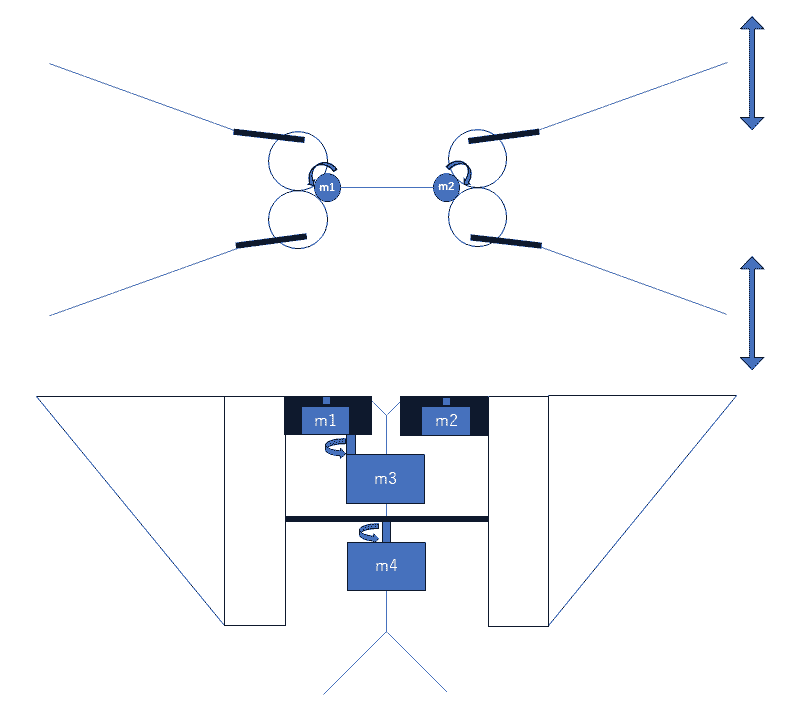
\includegraphics[width=\columnwidth]{modeling.png}
    \caption{The mechanical structure model of a tailless aerial robotic flapper. It has motors for thrust (m1, m2), a motor for pitch control (m3), and a motor for yaw control (m4).}
    \label{figure:modeling}
  \end{figure}
There are various types of flapping-wing drones, and we focus on a tailless aerial robotic flapper model\cite{karasek2018tailless}, as shown in Fig.~\ref{figure:modeling}.
The drone is mounted with four motors: two motors for thrust (m1, m2), one motor for pitch control (m3), and one motor for yaw control (m4).
We can treat the dynamics as a single rigid body as follows:
\begin{equation}
    \begin{aligned}
      &ma = mg + f\\
      &I\dot{\bm{\omega}} + \bm{\omega} \times I\bm{\omega} = \bm{\tau}
    \end{aligned}
\end{equation}
where $m$ is the mass of the drone, $a$ is the acceleration of the drone in the z direction, $g$ is the gravitational acceleration, $f$ is the thrust force, $I$ is the inertia matrix of the drone, \bm{$\omega$} is the $R^3$ angular velocity of the drone, and \bm{$\tau$} is the $R^3$ torque applied to the drone.
The thrust force $f$ and the torque $\bm{\tau}$ can be represented as follows:
\begin{equation}
  \label{eq:control}
  \begin{aligned}
    \begin{bmatrix}
      f\\
      \bm{\tau}
    \end{bmatrix}
    &=
    g(x_1, x_2, x_3, x_4)\\
    x_1 &= m_1\omega_1&
    x_2 = m_2\omega_2\\
    x_3 &= m_3\theta_3&
    x_4 = m_4\theta_4
  \end{aligned}
\end{equation}
where $\omega_i$ is the angular velocity of the motor $i$, $m_i$ is the coefficient of the motor $i$, $\theta_i$ is the angle of the motor $i$, and $g$ is the mapping function from $R^4$ to $R^4$.
Based on these equations, we can derive the following PID control law:
\begin{equation}
  \begin{aligned}
    &f_d = {PID}_r(e_r)
    &\bm{\tau}_d &= {PID}_R(\bm{e}_R)\\
    &e_r = r - r_d
    &\bm{e}_R &= R - R_d\\
  \end{aligned}
\end{equation}
where $f_d$ is the desired thrust force, 
$\bm{\tau}_d$ is the desired torque, 
$PID_r$ is the PID controller for the position, 
$PID_R$ is the PID controller for the orientation, 
$e_r$ is the error of the position, 
$\bm{e}_R$ is the error of the orientation, 
$R$ is the $R^3$ orientation of the drone, 
and $R_d$ is the desired orientation of the drone.
Then, we can calculate the desired motor inputs from the desired thrust force and torque using the inverse of Eq.~\ref{eq:control}.